% REV01 Sun 27 Jun 2021 10:31:25 WIB
% START Tue 04 May 2021 13:55:16 WIB

\chapter{A RUNAWAY MATCH}

Cherubic Pa arose with as little noise as possible from beside majestic
Ma, one morning early, having a holiday before him. Pa and the lovely
woman had a rather particular appointment to keep.

Yet Pa and the lovely woman were not going out together. Bella was up
before four, but had no bonnet on. She was waiting at the foot of the
stairs--was sitting on the bottom stair, in fact--to receive Pa when he
came down, but her only object seemed to be to get Pa well out of the
house.

‘Your breakfast is ready, sir,’ whispered Bella, after greeting him with
a hug, ‘and all you have to do, is, to eat it up and drink it up, and
escape. How do you feel, Pa?’

‘To the best of my judgement, like a housebreaker new to the business,
my dear, who can’t make himself quite comfortable till he is off the
premises.’

Bella tucked her arm in his with a merry noiseless laugh, and they went
down to the kitchen on tiptoe; she stopping on every separate stair to
put the tip of her forefinger on her rosy lips, and then lay it on his
lips, according to her favourite petting way of kissing Pa.

‘How do YOU feel, my love?’ asked R. W., as she gave him his breakfast.

‘I feel as if the Fortune-teller was coming true, dear Pa, and the fair
little man was turning out as was predicted.’

‘Ho! Only the fair little man?’ said her father.

Bella put another of those finger-seals upon his lips, and then said,
kneeling down by him as he sat at table: ‘Now, look here, sir. If you
keep well up to the mark this day, what do you think you deserve?
What did I promise you should have, if you were good, upon a certain
occasion?’

‘Upon my word I don’t remember, Precious. Yes, I do, though. Wasn’t
it one of these beau--tiful tresses?’ with his caressing hand upon her
hair.

‘Wasn’t it, too!’ returned Bella, pretending to pout. ‘Upon my word! Do
you know, sir, that the Fortune-teller would give five thousand guineas
(if it was quite convenient to him, which it isn’t) for the lovely piece
I have cut off for you? You can form no idea, sir, of the number of
times he kissed quite a scrubby little piece--in comparison--that I cut
off for HIM. And he wears it, too, round his neck, I can tell you! Near
his heart!’ said Bella, nodding. ‘Ah! very near his heart! However, you
have been a good, good boy, and you are the best of all the dearest boys
that ever were, this morning, and here’s the chain I have made of
it, Pa, and you must let me put it round your neck with my own loving
hands.’

As Pa bent his head, she cried over him a little, and then said (after
having stopped to dry her eyes on his white waistcoat, the discovery of
which incongruous circumstance made her laugh): ‘Now, darling Pa,
give me your hands that I may fold them together, and do you say after
me:--My little Bella.’

‘My little Bella,’ repeated Pa.

‘I am very fond of you.’

‘I am very fond of you, my darling,’ said Pa.

‘You mustn’t say anything not dictated to you, sir. You daren’t do it in
your responses at Church, and you mustn’t do it in your responses out of
Church.’

‘I withdraw the darling,’ said Pa.

‘That’s a pious boy! Now again:--You were always--’

‘You were always,’ repeated Pa.

‘A vexatious--’

‘No you weren’t,’ said Pa.

‘A vexatious (do you hear, sir?), a vexatious, capricious, thankless,
troublesome, Animal; but I hope you’ll do better in the time to come,
and I bless you and forgive you!’ Here, she quite forgot that it was
Pa’s turn to make the responses, and clung to his neck. ‘Dear Pa, if you
knew how much I think this morning of what you told me once, about the
first time of our seeing old Mr Harmon, when I stamped and screamed
and beat you with my detestable little bonnet! I feel as if I had been
stamping and screaming and beating you with my hateful little bonnet,
ever since I was born, darling!’

‘Nonsense, my love. And as to your bonnets, they have always been nice
bonnets, for they have always become you--or you have become them;
perhaps it was that--at every age.’

‘Did I hurt you much, poor little Pa?’ asked Bella, laughing
(notwithstanding her repentance), with fantastic pleasure in the
picture, ‘when I beat you with my bonnet?’

‘No, my child. Wouldn’t have hurt a fly!’

‘Ay, but I am afraid I shouldn’t have beat you at all, unless I had
meant to hurt you,’ said Bella. ‘Did I pinch your legs, Pa?’

‘Not much, my dear; but I think it’s almost time I--’

‘Oh, yes!’ cried Bella. ‘If I go on chattering, you’ll be taken alive.
Fly, Pa, fly!’

So, they went softly up the kitchen stairs on tiptoe, and Bella with
her light hand softly removed the fastenings of the house door, and Pa,
having received a parting hug, made off. When he had gone a little way,
he looked back. Upon which, Bella set another of those finger seals upon
the air, and thrust out her little foot expressive of the mark. Pa, in
appropriate action, expressed fidelity to the mark, and made off as fast
as he could go.

Bella walked thoughtfully in the garden for an hour and more, and then,
returning to the bedroom where Lavvy the Irrepressible still slumbered,
put on a little bonnet of quiet, but on the whole of sly appearance,
which she had yesterday made. ‘I am going for a walk, Lavvy,’ she said,
as she stooped down and kissed her. The Irrepressible, with a bounce in
the bed, and a remark that it wasn’t time to get up yet, relapsed into
unconsciousness, if she had come out of it.

Behold Bella tripping along the streets, the dearest girl afoot under
the summer sun! Behold Pa waiting for Bella behind a pump, at least
three miles from the parental roof-tree. Behold Bella and Pa aboard an
early steamboat for Greenwich.

Were they expected at Greenwich? Probably. At least, Mr John Rokesmith
was on the pier looking out, about a couple of hours before the coaly
(but to him gold-dusty) little steamboat got her steam up in London.
Probably. At least, Mr John Rokesmith seemed perfectly satisfied when
he descried them on board. Probably. At least, Bella no sooner stepped
ashore than she took Mr John Rokesmith’s arm, without evincing surprise,
and the two walked away together with an ethereal air of happiness
which, as it were, wafted up from the earth and drew after them a gruff
and glum old pensioner to see it out. Two wooden legs had this gruff and
glum old pensioner, and, a minute before Bella stepped out of the boat,
and drew that confiding little arm of hers through Rokesmith’s, he had
had no object in life but tobacco, and not enough of that. Stranded was
Gruff and Glum in a harbour of everlasting mud, when all in an instant
Bella floated him, and away he went.

Say, cherubic parent taking the lead, in what direction do we steer
first? With some such inquiry in his thoughts, Gruff and Glum, stricken
by so sudden an interest that he perked his neck and looked over the
intervening people, as if he were trying to stand on tiptoe with his two
wooden legs, took an observation of R. W. There was no ‘first’ in the
case, Gruff and Glum made out; the cherubic parent was bearing down and
crowding on direct for Greenwich church, to see his relations.

For, Gruff and Glum, though most events acted on him simply as
tobacco-stoppers, pressing down and condensing the quids within him,
might be imagined to trace a family resemblance between the cherubs in
the church architecture, and the cherub in the white waistcoat. Some
remembrance of old Valentines, wherein a cherub, less appropriately
attired for a proverbially uncertain climate, had been seen conducting
lovers to the altar, might have been fancied to inflame the ardour of
his timber toes. Be it as it might, he gave his moorings the slip, and
followed in chase.

The cherub went before, all beaming smiles; Bella and John Rokesmith
followed; Gruff and Glum stuck to them like wax. For years, the wings
of his mind had gone to look after the legs of his body; but Bella had
brought them back for him per steamer, and they were spread again.

He was a slow sailer on a wind of happiness, but he took a cross cut
for the rendezvous, and pegged away as if he were scoring furiously
at cribbage. When the shadow of the church-porch swallowed them up,
victorious Gruff and Glum likewise presented himself to be swallowed up.
And by this time the cherubic parent was so fearful of surprise, that,
but for the two wooden legs on which Gruff and Glum was reassuringly
mounted, his conscience might have introduced, in the person of that
pensioner, his own stately lady disguised, arrived at Greenwich in a
car and griffins, like the spiteful Fairy at the christenings of the
Princesses, to do something dreadful to the marriage service. And truly
he had a momentary reason to be pale of face, and to whisper to Bella,
‘You don’t think that can be your Ma; do you, my dear?’ on account of
a mysterious rustling and a stealthy movement somewhere in the remote
neighbourhood of the organ, though it was gone directly and was heard no
more. Albeit it was heard of afterwards, as will afterwards be read in
this veracious register of marriage.

Who taketh? I, John, and so do I, Bella. Who giveth? I, R. W. Forasmuch,
Gruff and Glum, as John and Bella have consented together in holy
wedlock, you may (in short) consider it done, and withdraw your two
wooden legs from this temple. To the foregoing purport, the Minister
speaking, as directed by the Rubric, to the People, selectly represented
in the present instance by G. and G. above mentioned.

And now, the church-porch having swallowed up Bella Wilfer for ever and
ever, had it not in its power to relinquish that young woman, but slid
into the happy sunlight, Mrs John Rokesmith instead. And long on the
bright steps stood Gruff and Glum, looking after the pretty bride, with
a narcotic consciousness of having dreamed a dream.

After which, Bella took out from her pocket a little letter, and read it
aloud to Pa and John; this being a true copy of the same.


‘DEAREST MA,

I hope you won’t be angry, but I am most happily married to Mr John
Rokesmith, who loves me better than I can ever deserve, except by loving
him with all my heart. I thought it best not to mention it beforehand,
in case it should cause any little difference at home. Please tell
darling Pa. With love to Lavvy,

Ever dearest Ma, Your affectionate daughter, BELLA (P.S.--Rokesmith).’


Then, John Rokesmith put the queen’s countenance on the letter--when had
Her Gracious Majesty looked so benign as on that blessed morning!--and
then Bella popped it into the post-office, and said merrily, ‘Now,
dearest Pa, you are safe, and will never be taken alive!’

Pa was, at first, in the stirred depths of his conscience, so far from
sure of being safe yet, that he made out majestic matrons lurking in
ambush among the harmless trees of Greenwich Park, and seemed to see a
stately countenance tied up in a well-known pocket-handkerchief glooming
down at him from a window of the Observatory, where the Familiars of the
Astronomer Royal nightly outwatch the winking stars. But, the minutes
passing on and no Mrs Wilfer in the flesh appearing, he became more
confident, and so repaired with good heart and appetite to Mr and Mrs
John Rokesmith’s cottage on Blackheath, where breakfast was ready.

A modest little cottage but a bright and a fresh, and on the snowy
tablecloth the prettiest of little breakfasts. In waiting, too, like
an attendant summer breeze, a fluttering young damsel, all pink and
ribbons, blushing as if she had been married instead of Bella, and yet
asserting the triumph of her sex over both John and Pa, in an exulting
and exalted flurry: as who should say, ‘This is what you must all come
to, gentlemen, when we choose to bring you to book.’ This same young
damsel was Bella’s serving-maid, and unto her did deliver a bunch of
keys, commanding treasures in the way of dry-saltery, groceries, jams
and pickles, the investigation of which made pastime after breakfast,
when Bella declared that ‘Pa must taste everything, John dear, or it
will never be lucky,’ and when Pa had all sorts of things poked into
his mouth, and didn’t quite know what to do with them when they were put
there.

Then they, all three, out for a charming ride, and for a charming stroll
among heath in bloom, and there behold the identical Gruff and Glum with
his wooden legs horizontally disposed before him, apparently sitting
meditating on the vicissitudes of life! To whom said Bella, in her
light-hearted surprise: ‘Oh! How do you do again? What a dear old
pensioner you are!’ To which Gruff and Glum responded that he see her
married this morning, my Beauty, and that if it warn’t a liberty he
wished her ji and the fairest of fair wind and weather; further, in a
general way requesting to know what cheer? and scrambling up on his two
wooden legs to salute, hat in hand, ship-shape, with the gallantry of a
man-of-warsman and a heart of oak.

It was a pleasant sight, in the midst of the golden bloom, to see this
salt old Gruff and Glum, waving his shovel hat at Bella, while his thin
white hair flowed free, as if she had once more launched him into blue
water again. ‘You are a charming old pensioner,’ said Bella, ‘and I am
so happy that I wish I could make you happy, too.’ Answered Gruff and
Glum, ‘Give me leave to kiss your hand, my Lovely, and it’s done!’ So it
was done to the general contentment; and if Gruff and Glum didn’t in the
course of the afternoon splice the main brace, it was not for want of
the means of inflicting that outrage on the feelings of the Infant Bands
of Hope.

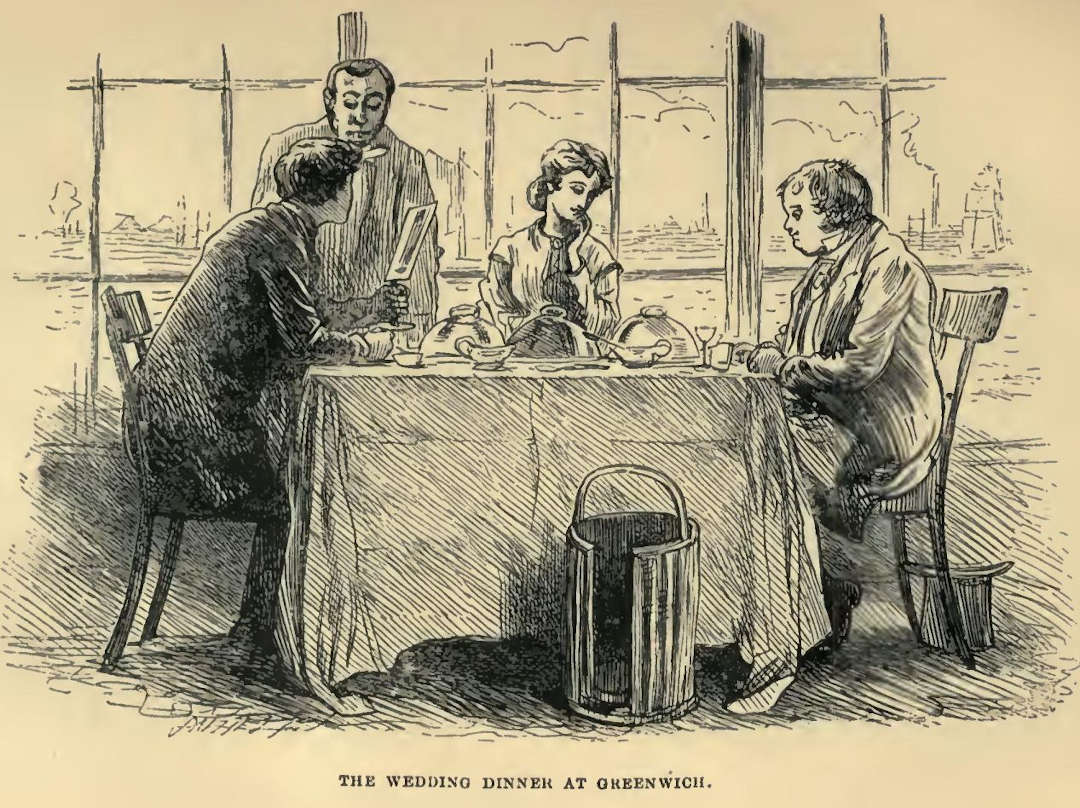
\includegraphics[scale=2.3]{04-04-01}

But, the marriage dinner was the crowning success, for what had bride
and bridegroom plotted to do, but to have and to hold that dinner in the
very room of the very hotel where Pa and the lovely woman had once dined
together! Bella sat between Pa and John, and divided her attentions
pretty equally, but felt it necessary (in the waiter’s absence before
dinner) to remind Pa that she was HIS lovely woman no longer.

‘I am well aware of it, my dear,’ returned the cherub, ‘and I resign you
willingly.’

‘Willingly, sir? You ought to be brokenhearted.’

‘So I should be, my dear, if I thought that I was going to lose you.’

‘But you know you are not; don’t you, poor dear Pa? You know that you
have only made a new relation who will be as fond of you and as thankful
to you--for my sake and your own sake both--as I am; don’t you, dear
little Pa? Look here, Pa!’ Bella put her finger on her own lip, and then
on Pa’s, and then on her own lip again, and then on her husband’s. ‘Now,
we are a partnership of three, dear Pa.’

The appearance of dinner here cut Bella short in one of her
disappearances: the more effectually, because it was put on under the
auspices of a solemn gentleman in black clothes and a white cravat, who
looked much more like a clergyman than THE clergyman, and seemed to
have mounted a great deal higher in the church: not to say, scaled the
steeple. This dignitary, conferring in secrecy with John Rokesmith on
the subject of punch and wines, bent his head as though stooping to
the Papistical practice of receiving auricular confession. Likewise,
on John’s offering a suggestion which didn’t meet his views, his face
became overcast and reproachful, as enjoining penance.

What a dinner! Specimens of all the fishes that swim in the sea, surely
had swum their way to it, and if samples of the fishes of divers
colours that made a speech in the Arabian Nights (quite a ministerial
explanation in respect of cloudiness), and then jumped out of the
frying-pan, were not to be recognized, it was only because they had all
become of one hue by being cooked in batter among the whitebait. And the
dishes being seasoned with Bliss--an article which they are sometimes
out of, at Greenwich--were of perfect flavour, and the golden drinks
had been bottled in the golden age and hoarding up their sparkles ever
since.

The best of it was, that Bella and John and the cherub had made a
covenant that they would not reveal to mortal eyes any appearance
whatever of being a wedding party. Now, the supervising dignitary, the
Archbishop of Greenwich, knew this as well as if he had performed the
nuptial ceremony. And the loftiness with which his Grace entered into
their confidence without being invited, and insisted on a show
of keeping the waiters out of it, was the crowning glory of the
entertainment.

There was an innocent young waiter of a slender form and with weakish
legs, as yet unversed in the wiles of waiterhood, and but too evidently
of a romantic temperament, and deeply (it were not too much to add
hopelessly) in love with some young female not aware of his merit.
This guileless youth, descrying the position of affairs, which even
his innocence could not mistake, limited his waiting to languishing
admiringly against the sideboard when Bella didn’t want anything, and
swooping at her when she did. Him, his Grace the Archbishop perpetually
obstructed, cutting him out with his elbow in the moment of success,
despatching him in degrading quest of melted butter, and, when by any
chance he got hold of any dish worth having, bereaving him of it, and
ordering him to stand back.

‘Pray excuse him, madam,’ said the Archbishop in a low stately voice;
‘he is a very young man on liking, and we DON’T like him.’

This induced John Rokesmith to observe--by way of making the thing more
natural--‘Bella, my love, this is so much more successful than any
of our past anniversaries, that I think we must keep our future
anniversaries here.’

Whereunto Bella replied, with probably the least successful attempt at
looking matronly that ever was seen: ‘Indeed, I think so, John, dear.’

Here the Archbishop of Greenwich coughed a stately cough to attract the
attention of three of his ministers present, and staring at them, seemed
to say: ‘I call upon you by your fealty to believe this!’

With his own hands he afterwards put on the dessert, as remarking to the
three guests, ‘The period has now arrived at which we can dispense with
the assistance of those fellows who are not in our confidence,’ and
would have retired with complete dignity but for a daring action issuing
from the misguided brain of the young man on liking. He finding, by
ill-fortune, a piece of orange flower somewhere in the lobbies now
approached undetected with the same in a finger-glass, and placed it on
Bella’s right hand. The Archbishop instantly ejected and excommunicated
him; but the thing was done.

‘I trust, madam,’ said his Grace, returning alone, ‘that you will have
the kindness to overlook it, in consideration of its being the act of a
very young man who is merely here on liking, and who will never answer.’

With that, he solemnly bowed and retired, and they all burst into
laughter, long and merry. ‘Disguise is of no use,’ said Bella; ‘they
all find me out; I think it must be, Pa and John dear, because I look so
happy!’

Her husband feeling it necessary at this point to demand one of those
mysterious disappearances on Bella’s part, she dutifully obeyed; saying
in a softened voice from her place of concealment:

‘You remember how we talked about the ships that day, Pa?’

‘Yes, my dear.’

‘Isn’t it strange, now, to think that there was no John in all the
ships, Pa?’

‘Not at all, my dear.’

‘Oh, Pa! Not at all?’

‘No, my dear. How can we tell what coming people are aboard the ships
that may be sailing to us now from the unknown seas!’

Bella remaining invisible and silent, her father remained at his
dessert and wine, until he remembered it was time for him to get home to
Holloway. ‘Though I positively cannot tear myself away,’ he cherubically
added, ‘--it would be a sin--without drinking to many, many happy
returns of this most happy day.’

‘Here! ten thousand times!’ cried John. ‘I fill my glass and my precious
wife’s.’

‘Gentlemen,’ said the cherub, inaudibly addressing, in his Anglo-Saxon
tendency to throw his feelings into the form of a speech, the boys down
below, who were bidding against each other to put their heads in the mud
for sixpence: ‘Gentlemen--and Bella and John--you will readily suppose
that it is not my intention to trouble you with many observations on the
present occasion. You will also at once infer the nature and even
the terms of the toast I am about to propose on the present occasion.
Gentlemen--and Bella and John--the present occasion is an occasion
fraught with feelings that I cannot trust myself to express. But
gentlemen--and Bella and John--for the part I have had in it, for the
confidence you have placed in me, and for the affectionate good-nature
and kindness with which you have determined not to find me in the way,
when I am well aware that I cannot be otherwise than in it more or less,
I do most heartily thank you. Gentlemen--and Bella and John--my love
to you, and may we meet, as on the present occasion, on many future
occasions; that is to say, gentlemen--and Bella and John--on many happy
returns of the present happy occasion.’

Having thus concluded his address, the amiable cherub embraced his
daughter, and took his flight to the steamboat which was to convey him
to London, and was then lying at the floating pier, doing its best to
bump the same to bits. But, the happy couple were not going to part with
him in that way, and before he had been on board two minutes, there they
were, looking down at him from the wharf above.

‘Pa, dear!’ cried Bella, beckoning him with her parasol to approach the
side, and bending gracefully to whisper.

‘Yes, my darling.’

‘Did I beat you much with that horrid little bonnet, Pa?’

‘Nothing to speak of; my dear.’

‘Did I pinch your legs, Pa?’

‘Only nicely, my pet.’

‘You are sure you quite forgive me, Pa? Please, Pa, please, forgive me
quite!’ Half laughing at him and half crying to him, Bella besought him
in the prettiest manner; in a manner so engaging and so playful and
so natural, that her cherubic parent made a coaxing face as if she had
never grown up, and said, ‘What a silly little Mouse it is!’

‘But you do forgive me that, and everything else; don’t you, Pa?’

‘Yes, my dearest.’

‘And you don’t feel solitary or neglected, going away by yourself; do
you, Pa?’

‘Lord bless you! No, my Life!’

‘Good-bye, dearest Pa. Good-bye!’

‘Good-bye, my darling! Take her away, my dear John. Take her home!’

So, she leaning on her husband’s arm, they turned homeward by a rosy
path which the gracious sun struck out for them in its setting. And O
there are days in this life, worth life and worth death. And O what a
bright old song it is, that O ‘tis love, ‘tis love, ‘tis love that makes
the world go round!



